% This is samplepaper.tex, a sample chapter demonstrating the
% LLNCS macro package for Springer Computer Science proceedings;
% Version 2.20 of 2017/10/04
%
\documentclass[runningheads]{llncs}
%
\usepackage{graphicx}
\usepackage{appendix}

% Used for displaying a sample figure. If possible, figure files should
% be included in EPS format.
%
% If you use the hyperref package, please uncomment the following line
% to display URLs in blue roman font according to Springer's eBook style:
% \renewcommand\UrlFont{\color{blue}\rmfamily}

\begin{document}
%
\title{The implication of the A* and PEA* algorithms in the 8-puzzle problem.\thanks{Degree in Software Engineering, University of Oviedo}}
%
%\titlerunning{Abbreviated paper title}
% If the paper title is too long for the running head, you can set
% an abbreviated paper title here
%
\author{Arroni del Riego, Sergio\orcidID{276341} \and
Galán Freire, Alejandro\orcidID{277346} \and
Antón de la Calle, Manuel \orcidID{276213}}
%
\authorrunning{Arroni del Riego, Sergio \and Galán Freire, Alejandro \and Antón de la Calle, Manuel}
% First names are abbreviated in the running head.
% If there are more than two authors, 'et al.' is used.
%
\institute{Oviedo University, Oviedo Asturias, Spain\\
\url{https://uniovi.es}}
%
\maketitle             % typeset the header of the contribution
%
\begin{abstract}
    Search algorithms are very important in Artificial Intelligence because they are the basis for many of the solutions in the different fields of Artificial Intelligence. In this work we will explain the A* and PEA* algorithms and we will compare them in the 8-puzzle problem. We will explain the differences between them.
    In addition, we will carry out an experimental study on the different heuristics we have used, which use the A* and PEA* algorithms. Finally, we will give our conclusion on the data obtained and we will say which is for us the better of the two algorithms. 

\keywords{A*  \and PEA* \and Search \and heuristic \and 8-puzzle \and IA \and Uniovi.}
\end{abstract}
%
%
%
\section{Introduction}
In this section, we will introduce the subject to be dealt with as well 
as a brief description of the rest of the sections of the work.

\subsection{Description of the topic to be addressed}
In this work we are going to apply the algorithm A* and PEA* to the 8-puzzle problem, 
for this we are going to use different heuristics.

\subsection{Description of the sections of the work}
In the following points we will discuss:
\begin{enumerate}
\setcounter{enumi}{1}
\item Description of the 8-puzzle problem, in this section we will detail how the problem in question works.
\item Description of the algorithms involved in the work, in this section we will explain in detail how the algorithms used work, as well as a brief state of the art of them.
\item Application of the algorithms to the 8-puzzle problem, we will explain the approach we have taken to the 8-puzzle problem, as well as the heuristics to be used, including the one we propose in this work.
\item Experimentation, we will compare $A^*$ and $PEA^*$ with various heuristics, as well as the one proposed in this work.
\item Conclusion, here we will give our critical opinion about this application of the two algorithms.
\end{enumerate}

\section{The 8-puzzle problem}
The 8-puzzle problem is well known and used for the study of search algorithms, informed or uninformed, 
generally of the second type, i.e., they also include the study of various heuristics that try to reach 
the objective state in the optimal way. However, heuristics can be applied simply with the intention to 
analyze it without the need for it to be good.

\subsection{Description of problem}
It is actually a concrete example of the n-puzzle problem, which is used because it is simple to understand 
at this size.

So, for this particular example, we have a 3x3 board where 8 of the cells are filled with all the numbers 
from 1 to 8 while one remains empty. This will be the one to which we have to move the cells in order to reach 
the desired final state.

There are 4 possible movements, displacement of a cell to its adjacent cell located in the north, south, east 
or west as long as the cell is empty in one of the locations. Figure \ref{fig1} shows three possible states.

The cost of each movement is 1, and the goal is to reach the target state by adding as few movements as possible 
and, therefore, achieving the lowest cost.

The target state that we will consider is as follows:
{1, 2, 3, 8, 0, 4, 7, 6, 5}

\subsection{Classic methods of resolution}
As I said at the beginning, the algorithms that can be used to solve this problem can be informed, such as algorithms 
$A^*$ and $PEA^*$, and not informed such as BFS (more information you can find in \cite{algorithms_2}).

We will study the application of the $A^*$ and $PEA^*$ algorithms with heuristics having different characteristics.

\begin{figure}
\centering
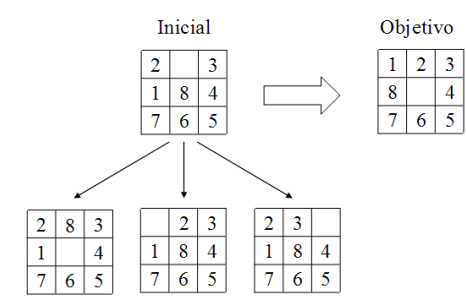
\includegraphics[width=0.65\textwidth]{8puzzle.png}
\caption{Figure showing the starting point, the objective and the stages we went through to achieve it.} \label{fig1}
\end{figure}

\section{The search algorithms}
In this section, we will discuss about search algorithms, doing a distinction between uninformed and informed search algorithms.
The uninformed algorithms that we will discuss are: Best First (\(BF\)).
The informed algorithms that we will discuss are: $A^*$ and $PEA^*$.

\subsection{Best first search (\(BF\))}
The uninformed search algorithms are those that do not use any information about the problem, they just expand the next node in the frontier.
The most important thing that differentiates the various uninformed algorithms is the method they use to expand the next node in the frontier.
Hereafter, we will trate the Best First (\(BF\)) search algorithm.

We will start with the "Best First" (\(BF\)) search algorithm \cite{algorithms}, which is the basis of informed search algorithms, such as \(A^*\).
\(BF\) is based on the idea of idea of expanding the node with the lowest cost. The cost of a node is calculated by the heuristic function \(h(n)\) used. \\
In the \(BF\) algorithm, we have two list, the list "open" that this list contains the nodes that are not expanded yet, and the list "closed" that contains the nodes that are expanded.

You can see a more detailed description and a implementation of the algorithm in Russell's and Norvig's book \cite{algorithms_2}.

\subsection{The \(A^*\) algorithm}
The informed search algorithms are those that use the any information about the problem to expand the next node in the frontier.\\
The \(A^*\) algorithm is a variation of the \(BF\) algorithm, this was proposed by Peter E. Hart, Nils J. Nilsson and Bertram Raphael in their work in 1968 \cite{algorithms_3}.\\
In \(A^*\), use a function \(f\) to evaluate the nodes, this function in \(A^*\) is representate by \(f^*(n)\) and this is the cost of the shortest path from initial to \(n\) conditional on passing through \(n\).
The function \(f^*(n)\) (where n is any node) is defined as equation \ref{eqn:a*}:

\begin{equation}\label{eqn:a*}
f^*(n) = g^*(n) + h^*(n)
\end{equation}

Where \(g^*(n)\) is the cost of the path from the initial node to the node \(n\), and \(h^*(n)\) is the heuristic function that estimates the cost of the path from the node \(n\) to the goal node, you can see this function in more detail in Nilsson's book "Principles of artificial intelligence" \cite{algorithms_4}.
In A* we talk about f*, g* and h*, but in most cases these are only estimates because it is very complicated for complex problems to know the exact values, if we knew them the algorithm would go straight to the goal. Instead we use the estimates f, g and h, so the function would be as we can see in equation \ref{eqn:a_2}:

\begin{equation}\label{eqn:a_2}
f(n) = g(n) + h(n)
\end{equation}

The \(A^*\) algorithm is as follows, we have two list, the list "open" that this list contains the nodes that are not expanded yet, and the list "closed" that contains the nodes that are expanded:

\begin{enumerate}
\item Initialises the "open" list with the start node.
\item Initialises the "closed" list with the empty list.
\item While the "open" list is not empty:
\begin{enumerate}
\item Select the node with the lowest cost, you can se the equation in \ref{eqn:a*}, in the "open" list and remove it from the "open" list.
\item If the node is the goal, stop.
\item If not, add the node to the "closed" list and expand its children.
\item For each child:
\begin{enumerate}
\item If the child is in the "closed" list, do nothing.
\item If the child is not in the "open" list, add it.
\item If the child is in the "open" list, but the \(f(child)\) is better than the previous path, replace the child in the "open" list with the new child.
\end{enumerate}
\end{enumerate}
\item Return to Step 3.
\end{enumerate}

One problem that have the \(A^*\) algorithm is that it can be very slow, because it can expand a lot of nodes, and this can be a problem if the problem has a lot of nodes. To solve this problem, we can use the $PEA^*$ algorithm.\\
If you want to see a more detailed description and a implementation of the algorithm, you can see Russell's and Norvig's book \cite{algorithms_2}.

\subsection{The \(PEA^*\) algorithm}
The \(PEA^*\) algorithm is a variation of the \(A^*\) algorithm, in fact it is faster than the base algorithm \(A^*\).
Is a not admitted algorithm, this means that it is not guaranteed to find the optimal solution, but it is very fast and useful in practice.
The algorithm have a function, very similar to the \(A^*\) function, but it is not the same, this function is called \(f_{PEA}^*(n)\) and is defined in equation \ref{eqn:pea*}:

\begin{equation}\label{eqn:pea*}
f_{PEA}^*(n) = g^*(n) + h^*(n) * (1 + \epsilon)
\end{equation}

Where \(g^*(n)\) is the cost of the path from the initial node to the node \(n\), 
\(h*(n)\) is the heuristic function that estimates the cost of the path from the node \(n\) to the goal node and 
\(\epsilon\) is a constant that is used to control the expansion of the nodes.\\
You can see this algorithm in more detail in Maria Rita's tesis \cite{algorithms_5}.

\section{Application of the $A^*$ and \(PEA^*\) algorithms to the 8-puzzle problem}
The state space of this problem is defined by the set of possible combinations on the board,
 i.e. the location of all the tiles.

$A^*$ is admissible when an admissible heuristic is applied to it, but 
$PEA^*$ is an $\varepsilon-admissible$ algorithm, which give up 
admissibility when the problem size is too large. Therefore, we will use 
different values of epsilon to be specified in the experimental study.

We will apply the same heuristics to both algorithms. They are the following:
\begin{enumerate}
    \item $h_1(n)$: number of tiles that are out of place.
    \item $h_2(n)$: sum of orthogonal distances from each tile to its final position.
    \item $h_3(n)$: $2*number$ of tiles at orthogonal distance 2 from their final position.
    \item $h_4(n)$: $h_2$ multiplied by 0.4 summed with $h_1$.
\end{enumerate}
\subsection{Properties of heuristics}
The first two heuristics are typical for solving the 8-puzzle problem with 
the $A^*$ algorithm. They are monotone by satisfying that their sequence of 
values f(n) of the expanded nodes is non-decreasing, and they also satisfy equation 
\ref{eqn:monotone}, and this also implies that they are admissible, 
i.e., they always reach the optimal solution.

\begin{equation}\label{eqn:monotone}
    h(n1) \leq h(n2) + c(n1,n2)
\end{equation}

On the other hand, from the book \cite{algorithms_2} we conclude that $h_2$  is the best heuristic since the ideal 
case is that the length of the trajectory to the target position is equal 
to the orthogonal distance of the token to its target. $h_2$ 
is more informed than the rest, i.e., it dominates the rest of heuristics 
tested for solving this problem, which means that all nodes expanded by $h_2$ 
will be expanded by the rest. It satisfies:

\begin{equation}\label{eqn:dominance}
    hx(n) < h2(n) \leq h^*(n)
\end{equation}

Also, we believe that $h_3$ also meets the characteristics 
of the first two heuristics because of the data obtained in the study 
shown in the next point of the practice. Anyway, it is not as good heuristic as $h_1$ and $h_2$.

Finally, $h_4$ is not monotonic because the $f(n)$ values of the expanded 
nodes is decreasing. Moreover, it is not admissible and we can make 
the following proof:

We know that $h_1$ and $h_2$ are admissible so they satisfy equantion \ref{eqn:admissible} for all values of $n$. If we then assume equation 
\ref{eqn:min_cost}, we have \ref{eqn:h4}, 
so it does not satisfy the admissibility condition. 

\begin{equation}\label{eqn:min_cost}
    h_1(n) = h_2(n) = h^*(n) = 1
\end{equation}

\begin{equation}\label{eqn:admissible}
    hx(n) \leq h^*(n)
\end{equation}

\begin{equation}\label{eqn:h4}
    h4(n) = 1 + 0.4*1 > h*(n)
\end{equation}

\section{Experimental study}
In this section, we will test the algorithms to see if the theory holds.
We will collect data for each algorithm separately, combining the different
heuristics with various board instances with increasing costs. We will proceed to
interpret the data to support or refute the theory and finally make a comparison between the two algorithms.
\subsection{Experimental study design}
To measure the differences between $A^*$ and \(PEA^*\) algorithms we will annotate 
the number of expanded nodes, re-expanded nodes, the cost, the number of moves and the time to finish.

With the \(PEA^*\) algorithm we will use an epsilon $\epsilon_1=0.01$, $\epsilon_2=10$ and $\epsilon_3=100$.
The algorithms are implemented in the AIMA3e project from the book \cite{algorithms_2} with a path cost function $f={cost}^{cost}$ and 
all heuristics will use the weighted version seen in the class $f={val}^{val}$ 
where val is the value of the tile to move.
The board instances we are going to test are of cost of 5, 15, 30 moves provided in the labs and now shown because of space limitation.

The computer is a quad-core Intel i7 CPU and 12GB of RAM.
\subsection{Experimental results}
The first tests are performed on the \(A^*\) algorithm using the different heuristics and board instances.

Table \ref{tab1} collects the costs and moves for each heuristic and show how $h_1$, $h_2$, $h_3$ are admissible and $h_4$ are not,
since the theory tells us that the first three always find the best solution and therefore the three must show the same, and $h_4$ an equal or higher cost.

Of the different heuristics tested, Figure \ref{fig2} shows that the one which gives the best results is $h_2$ since it offers shorter times than the rest,
expands fewer nodes (the graph not drew due to space limitation) and finds the best solution, followed in second place by $h_1$.

\begin{table}[!htb]
    \begin{minipage}{.5\linewidth}
      \centering
      \begin{tabular}{|l|l|l|}
        \hline
        Heuristic & Path cost & Moves\\
        \hline
        $h_1$ & 3,1119E+14 & 15\\
        $h_2$ & 3,1119E+14 & 15\\
        $h_3$ & 3,1119E+14 & 15\\
        $h_4$ & 3,11474E+14 & 24\\
        \hline
        \end{tabular}
    \end{minipage}%
    \begin{minipage}{.5\linewidth}
      \centering
        \begin{tabular}{|l|l|l|}
            \hline
            Heuristic & Path cost & Moves\\
            \hline
            $h_1$ & 1,53474E+14    & 31\\
            $h_2$ & 1,53474E+14    & 31\\
            $h_3$ & 1,53474E+14    & 31\\
            $h_4$ & 1,53743E+14    & 35\\
            \hline
            \end{tabular}
    \end{minipage} 
    \caption{Average path costs and moves for each heueristics using A* with board instances of 15 (left) and 30 (right).}\label{tab1}
\end{table}
\begin{figure}
    \centering
    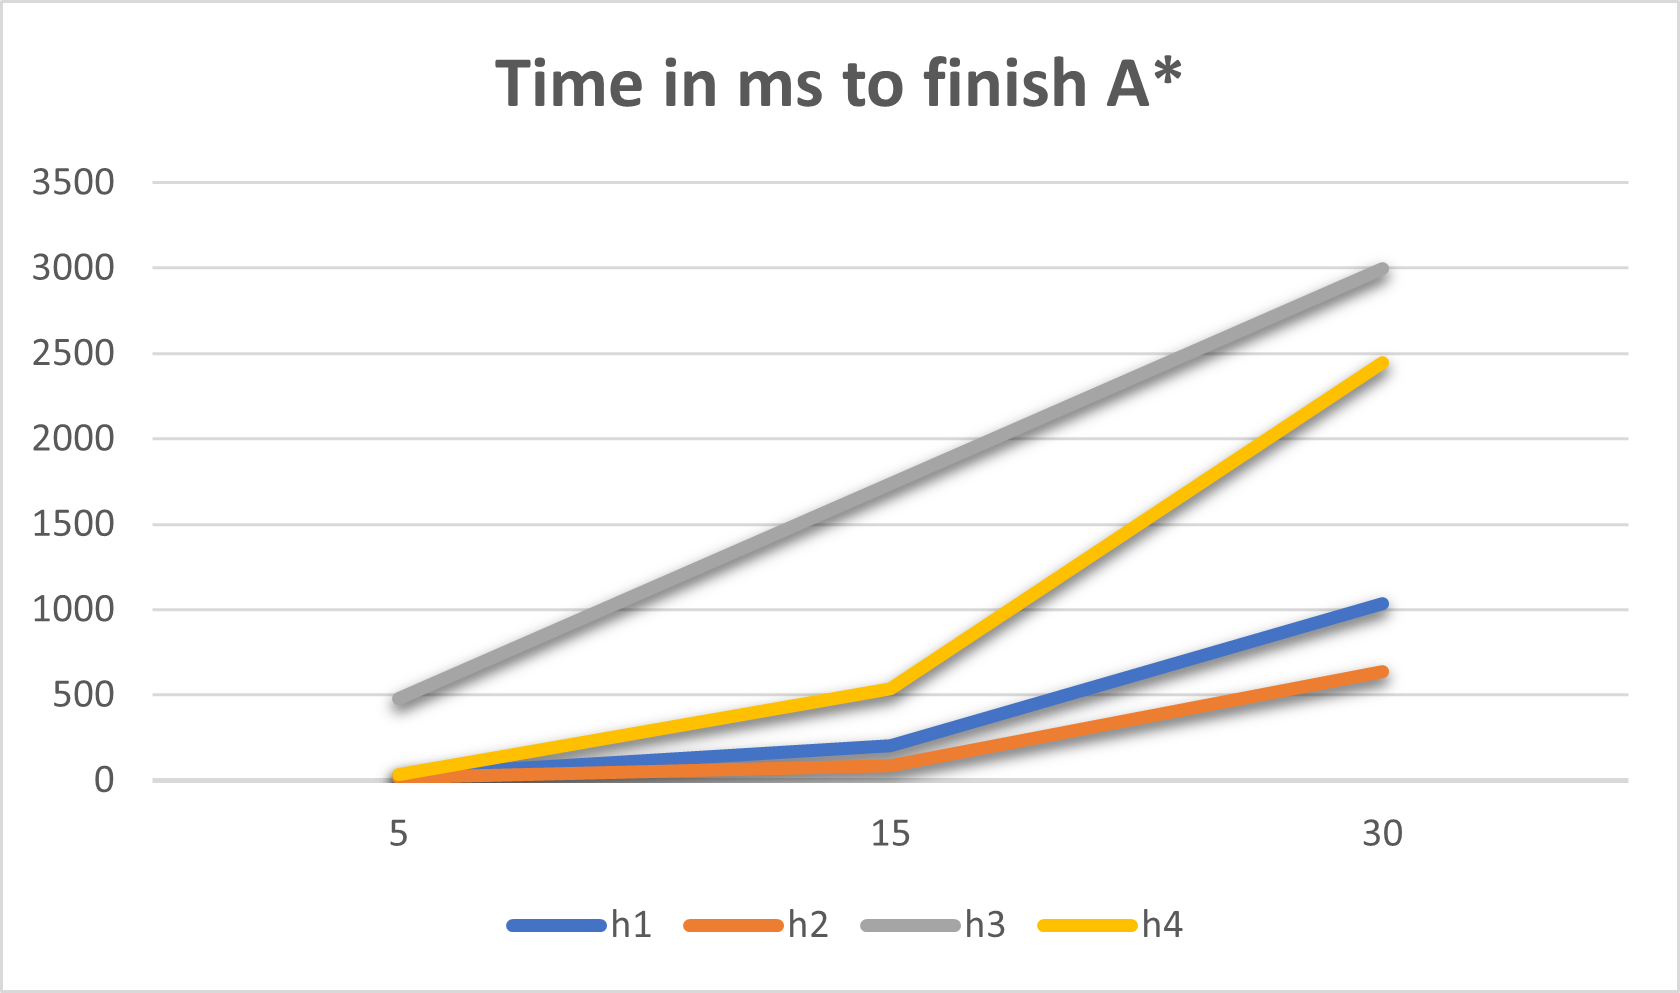
\includegraphics[width=0.65\textwidth]{seconds_A.png}
    \caption{Time in ms to resolve the problem for each heuristic with $A^*$ algorithm.} \label{fig2}
\end{figure}
Also, as demonstrated in Section 4, the heuristics $h_3$ and $h_4$ are not monotonic and consistent so they can re-expand nodes, this result is reflected in Table \ref{tab3}.
\begin{table}
    \centering
    \begin{tabular}{|l|l|l|}
    \hline
    Heuristic & Cost 15 & Cost 30\\
    \hline
    $h_1$ & 0 & 0\\
    $h_2$ & 0 & 0\\
    $h_3$ & 82680 & 129155 \\
    $h_4$ & 90 & 9982\\
    \hline
    \end{tabular}
    \caption{Nodes re-expanded for each heuristic using $A^*$ and the board instances (\{7, 0, 3, 5, 1, 8, 2, 6, 4\}) and (\{5, 6, 7, 4, 0, 8, 3, 2, 1\}) of cost 15 and 30 respectively. }\label{tab3}
\end{table}

We now continue with the $PEA^*$ algorithm.
The results of the costs from the solutions found by $PEA^*$ collected in Table \ref{tab2}
show how the algorithm is inadmissible, since, the costs obtained are equal to or higher than the costs in Table \ref{tab1}.

\begin{table}[!htb]
    \caption{Average path costs and moves for each heueristics using $PEA^*$, $\epsilon=10$ and with board instances of 15 (left) and 30 (right).}\label{tab2}
    \begin{minipage}{.5\linewidth}
      \centering
      \begin{tabular}{|l|l|l|}
        \hline
        Heuristic & Path cost & Moves\\
        \hline
        $h_1$ & 3,11474E+14    & 24\\
        $h_2$ & 3,95828E+14    & 28\\
        $h_3$ & 4,83597E+14    & 25\\
        $h_4$ & 3,96344E+14    & 33.5\\
        \hline
        \end{tabular}
    \end{minipage}%
    \begin{minipage}{.5\linewidth}
      \centering
        \begin{tabular}{|l|l|l|}
            \hline 
            Heuristic & Path cost & Moves\\
            \hline
            $h_1$ & 1,53510E+14    & 36\\
            $h_2$ & 2,46159E+14    & 42\\
            $h_3$ & 4,04707E+14    & 30\\
            $h_4$ & 4,05508E+14    & 44.5\\
            \hline
            \end{tabular}
    \end{minipage} 
\end{table}


Next, let's compare the two algorithms.
$PEA^*$ is used to decrease times and number of nodes expanded
with respect to $A^*$ in exchange for not finding the best solution (not admissible) so,
we will compare it with the best heuristic of $A^*$, i.e., we will compare it with $h_2$.

Figures \ref{fig4} show how for more complicated board configurations the $PEA^*$ algorithm gives
better performance than $A^*$.
It highlights how $\epsilon=100$ offers better performance in these tests.

\begin{figure}
    \centering
    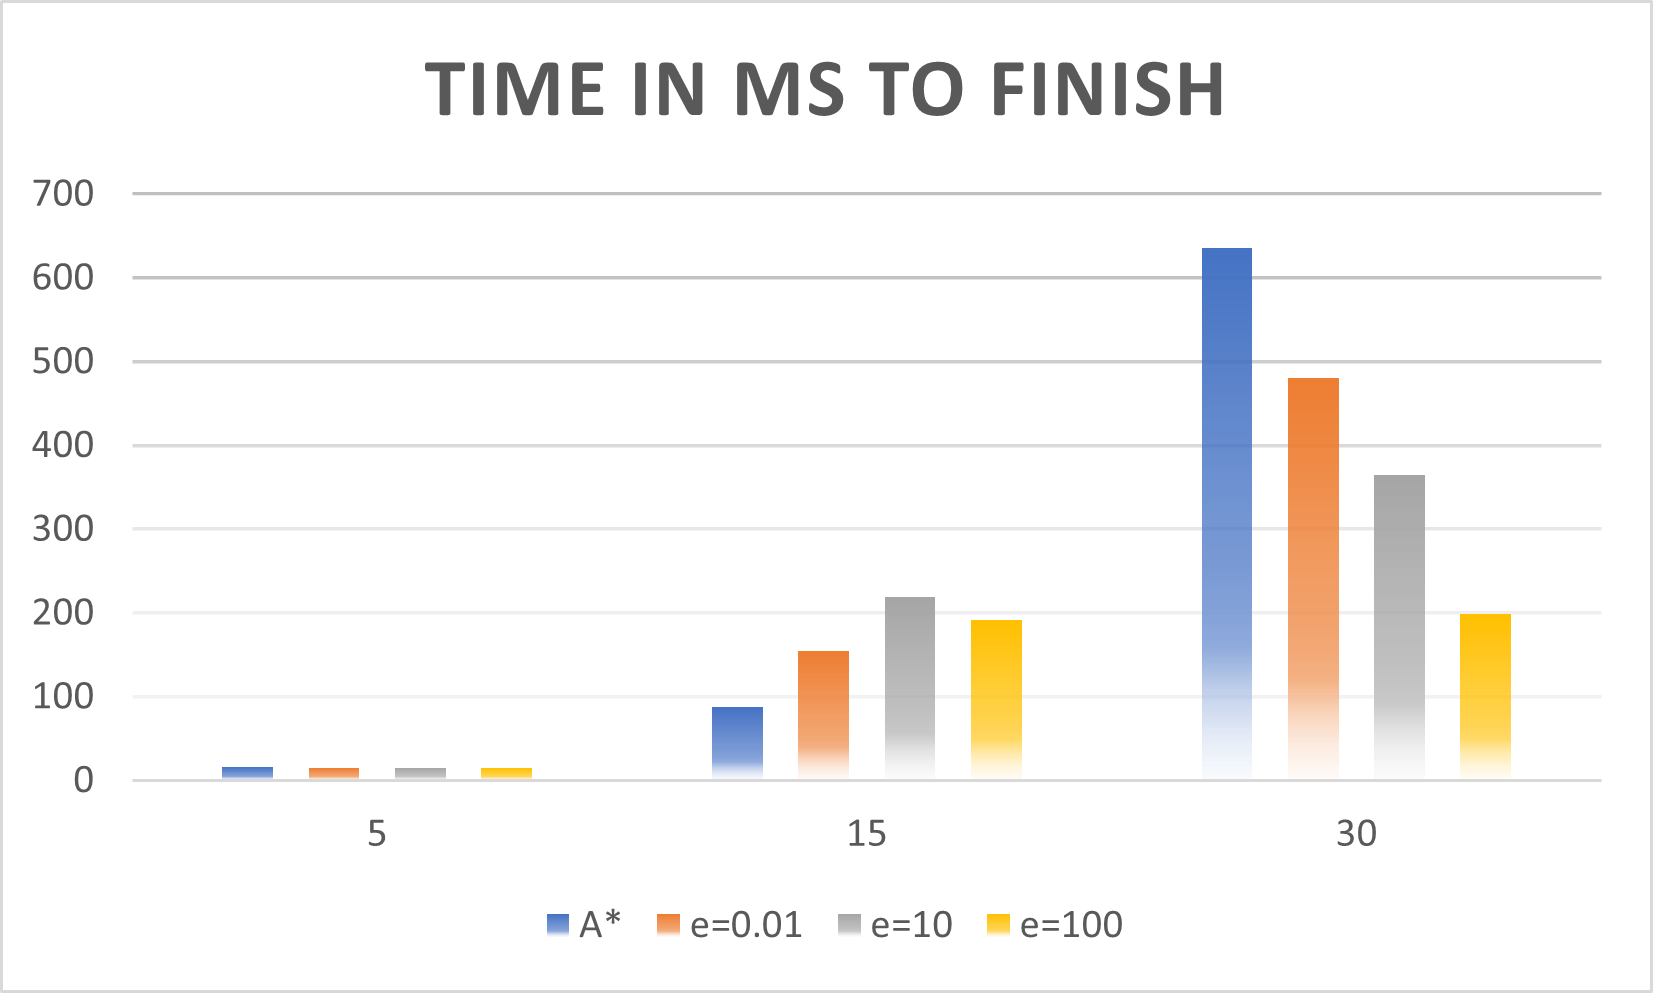
\includegraphics[width=0.65\textwidth]{time_AvsPEA.png}
    \caption{Time in ms to resolve the problem for each epsilon with $PEA^*$ algorithm and $h_2$.} \label{fig4}
\end{figure}
\section{Conclusions}
After all the tests we can observe $A^*$ always finds the optimal solution, while sometimes 
$PEA^*$ does not achieve it (not even reaching the target state) increasing 
the number of moves to perform and the cost while decreasing the time spent 
as well as the number of expanded nodes. We also note that among the epsilon 
values tested (0.01, 10, 100) the one that gives the best results is 100.

As for the heuristics, according to the study carried out, the best is $h_2$, 
expanding fewer nodes than the rest as it is more informed and always obtaining 
the optimal solution, the latter as well as $h_1$ and $h_3$. The worst of all we 
see is $h_4$, not being admissible and in the results not reaching the best possible 
solution in one of the occasions.

We conclude that the best algorithm is $A^*$ because in this problem time is not
a problematic factor since it moves between values of a few ms to 4 seconds and
$PEA^*$ offers a small improvement compared to the increase of movements it generates.

\bibliography{refs} 
\bibliographystyle{ieeetr} 
\appendix
\chapter*{Annex 1: Work Distribution}
Arroni del Riego, Sergio\orcidID{Uo276341}: I realize the Introduction, A*, PEA*, and BF algorithms explication, Abstract, and KeyWords.\\
Galán Freire, Alejandro\orcidID{Uo277346}: I realize the 8-puzzle problem explication, the application of the A* and PEA* algorithms to the 8-puzzle problem, and conclusions.\\
Antón de la Calle, Manuel\orcidID{Uo276213}: I realize the Experimental study.\\
All: All of us did the tasks of writing in English and using LaTex for the writing of the work.
\end{document}
